%%%%%%%%%%%%%%%%%%%%%%%%%%%%%%%%%%%%%%%%%%%%%%%%%%%
%                                                 %
%                     SECTION                     %
%                                                 %
%%%%%%%%%%%%%%%%%%%%%%%%%%%%%%%%%%%%%%%%%%%%%%%%%%%

\section{Apparatus}
\label{sec:sec005}

For the material and apparatus, it is essential to capture the session apprehending the user interactions. In our case, we will record this interaction by using the \hyperlink{https://support.apple.com/quicktime}{QuickTime Player Version 10.4 (928.5.1)} to obtain all interactions. We will pair this video tool with a user watch tool called \hyperlink{https://www.hotjar.com/}{Hotjar} and an eye tracker. The \hyperlink{https://www.hotjar.com/}{Hotjar} tool serves the purpose of using several logs of the interaction and gives us visualization over it. The eye tracker will be the \hyperlink{https://gaming.tobii.com/product/tobii-eye-tracker-4c/}{Tobii Eye Tracker 4C} (SN: IS404-100107008875) device. All instruments will help us to capture where and when are users interacting. By looking at the test participant's reactions, we find a lot of information regarding the prototype design.

The tools that we choose for the material and apparatus of this User Testing Guide are low-cost and easy to use. Our equipment is a cost-effective and, by using our laboratory materials, bringing it to the RR, we enable to capture not only what the user is doing on the screen, but on the body language supported by the interviews and observations.

\hfill

The material used in the test sessions for the user interface consists of:

\begin{itemize}
\item MacBook Pro: it will allow the user to interact with the keyboard and a wireless mouse;
\item Wireless Mouse: it will allow the user to interact with a mouse and will complement the keyboard;
\end{itemize}

%%%%%%%%%%%%%%%%%%%%%%%%%%%%%%%%%%%%%%%%%%%%%%%%%%%
%                                                 %
%                     SECTION                     %
%                                                 %
%%%%%%%%%%%%%%%%%%%%%%%%%%%%%%%%%%%%%%%%%%%%%%%%%%%

\subsection{Technical Details}

To produce this traditional environment, and since we can simulate with a laptop, the mouse and keyboard interaction, we are using a Microsoft Mobile Mouse 4000 together with the \hyperlink{https://www.apple.com/shop/buy-mac/macbook-pro}{MacBook Pro} (Retina, 13-inch, Early 2016) with a standard integrated keyboard on the laptop.

%%%%%%%%%%%%%%%%%%%%%%%%%%%%%%%%%%%%%%%%%%%%%%%%%%%
%                                                 %
%                     SECTION                     %
%                                                 %
%%%%%%%%%%%%%%%%%%%%%%%%%%%%%%%%%%%%%%%%%%%%%%%%%%%

\subsection{Devices}

Traditional interaction remains the most common way to interact with user interfaces in a clinical environment. Unfortunately, most of this interaction is made by low profile equipment that makes users produce more errors and take more time interacting with those User Interfaces (UI)~\cite{lopes2018interaction, paulo3d, sousa2017vrrrroom}.

For this \textit{User Testing Guide}, we will use the \hyperlink{https://gaming.tobii.com/product/tobii-eye-tracker-4c/}{Tobii Eye Tracker 4C} (\hyperlink{https://www.tobii.com/}{Tobii}, Sweden). This device, is a remote eye tracking device that provides an estimate of the point-gaze and 3D eye position for each eye at 90Hz~\cite{di2014saccadic, marandi2018eye, marandi2018reliability}. We will attach the eye tracker under the display area with a magnetic mounting bracket, following the product's instructions. A 9-point calibration~\cite{chatelain2018evaluation} will be performed for each user. Our protocol was implemented in \hyperlink{https://www.python.org/}{Python} (\textit{versions} $\geqslant$ \hyperlink{https://docs.python.org/2/}{v2.7}) and \hyperlink{http://www.processing.org/}{Processing} (\textit{versions} $\geqslant$ \hyperlink{https://github.com/processing/processing/releases/tag/processing-0269-3.5.3}{v3.5.3}). The setup repository was the \hyperlink{https://github.com/mida-project/eye-tracker-setup}{eye-tracker-setup}, while the repository to measure and calculate the setup gazing information was the \hyperlink{https://github.com/mida-project/eye-tracker-naive}{eye-tracker-naive} repository.

%%%%%%%%%%%%%%%%%%%%%%%%%%%%%%%%%%%%%%%%%%%%%%%%%%%
%                                                 %
%                     SECTION                     %
%                                                 %
%%%%%%%%%%%%%%%%%%%%%%%%%%%%%%%%%%%%%%%%%%%%%%%%%%%

\subsection{User Interactions}

The systems have several buttons (Figure \ref{fig:toolbar}) that allows the user to interact or access to a set of user interface features. Each item of the following list represents each metaphoric icon of Figure \ref{fig:toolbar}.

%%%%%%%%%%%%%%%%%%%%%%%%%%%%%%%%%%%%%%%%%%%%%%%%%%%

\hfill

\begin{figure}[h]
\centering

\includegraphics[width=\textwidth]{toolbar}
\caption{Toolbar of the System available features.}
\label{fig:toolbar}
\end{figure}

\hfill

%%%%%%%%%%%%%%%%%%%%%%%%%%%%%%%%%%%%%%%%%%%%%%%%%%%

The buttons are (from left to right of Figure \ref{fig:toolbar}) as follows:

\hfill

\begin{itemize}
\item WW/WC
\item Invert
\item Zoom
\item Pan
\item Stack Scroll
\item Freehand
\item Probe
\item Save
\item Window Controller
\end{itemize}

\hfill

%%%%%%%%%%%%%%%%%%%%%%%%%%%%%%%%%%%%%%%%%%%%%%%%%%%
%                                                 %
%                     SECTION                     %
%                                                 %
%%%%%%%%%%%%%%%%%%%%%%%%%%%%%%%%%%%%%%%%%%%%%%%%%%%

On Figure \ref{fig:patient_list}, the user can select the list of patients. The list has a table with several patient information. The first column is the \textit{Patient ID}; we used it as an identifier of the patient. In that way, we can have anonymized information with no reference to the patient name. The second column is the \textit{Study Date}, the third column is the \textit{Modality} of the used \textbf{DICOM} image, the fourth column is the \textit{Study Description} of the used study and the last column is the number of \textit{Images}.

\clearpage

%%%%%%%%%%%%%%%%%%%%%%%%%%%%%%%%%%%%%%%%%%%%%%%%%%%

\hfill

\begin{figure}[h]
\centering
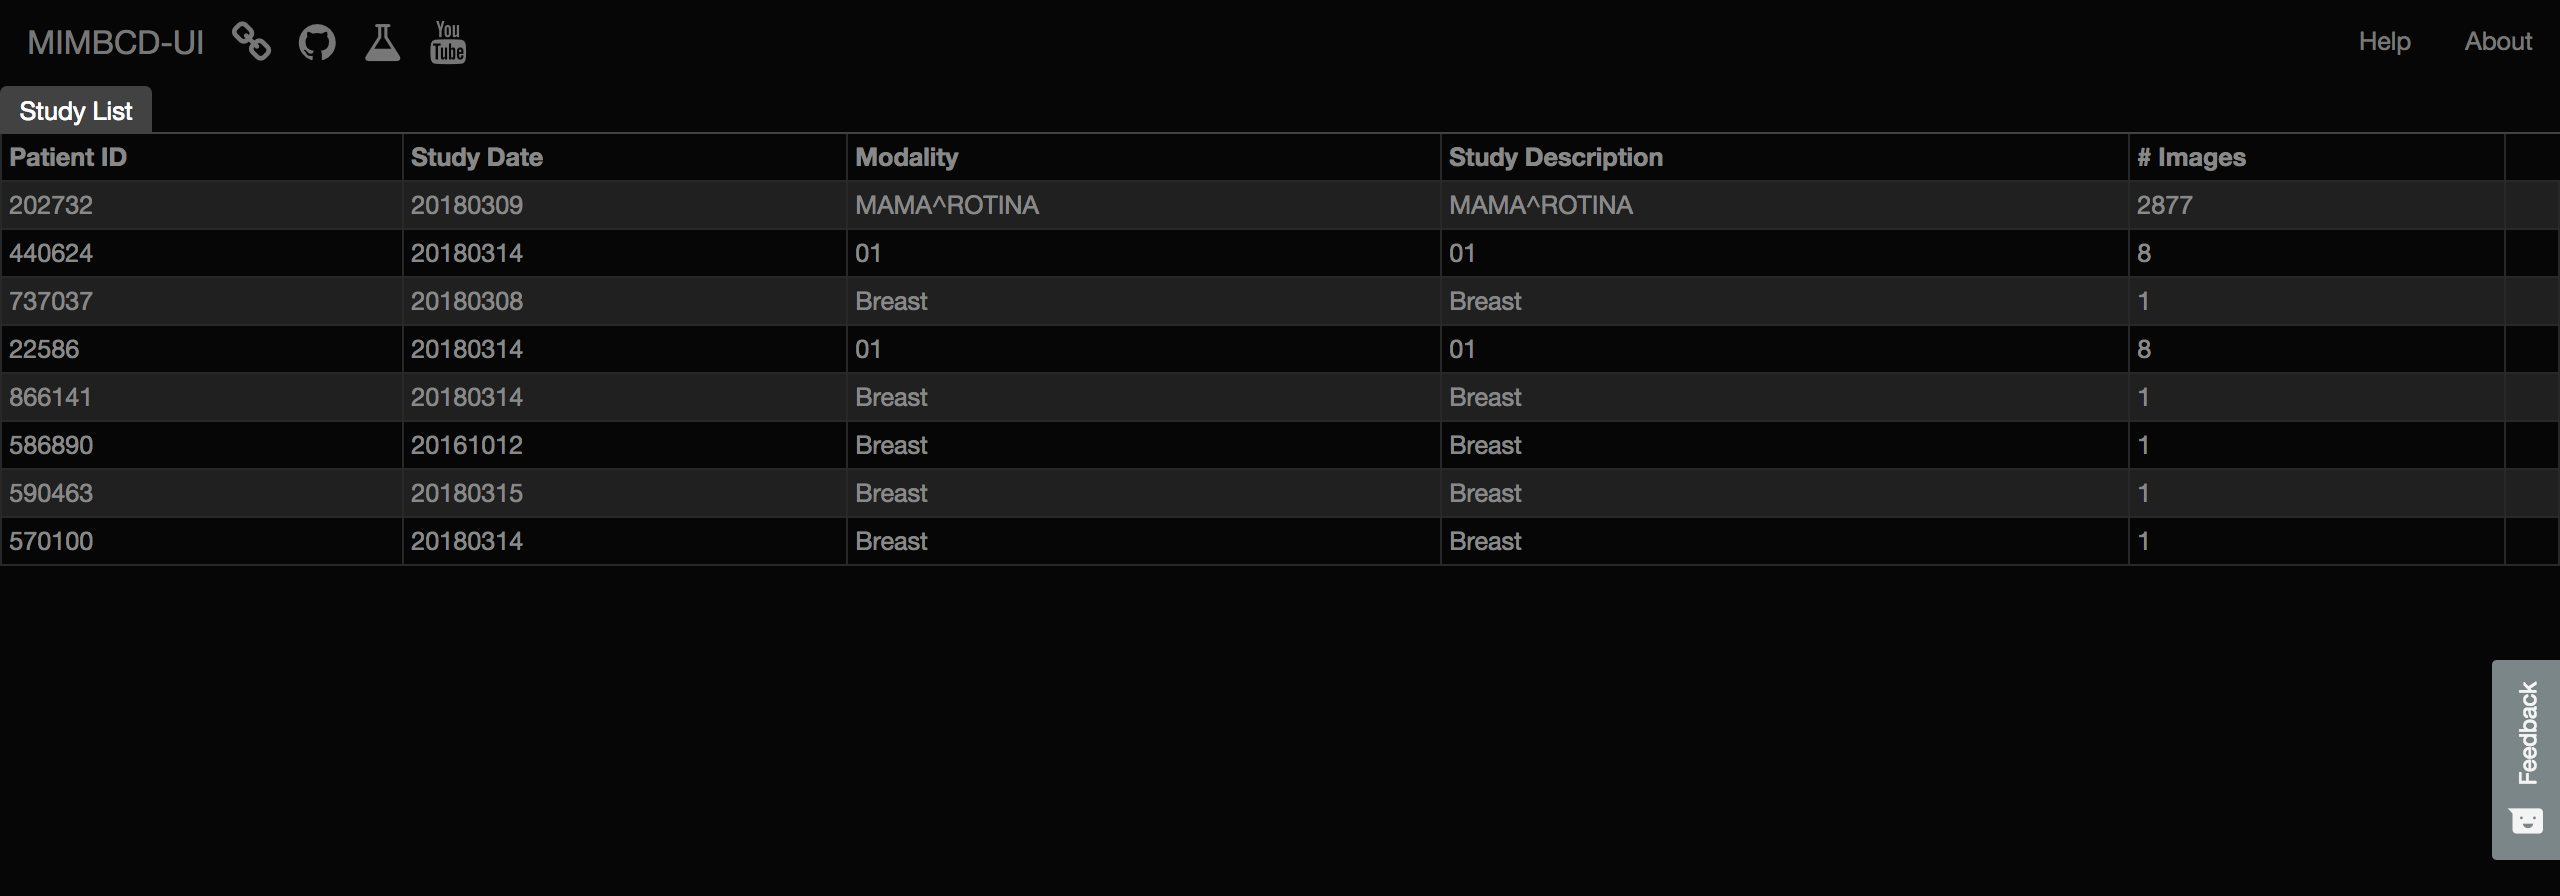
\includegraphics[width=\textwidth]{patient_list}
\caption{List of Patients.}
\label{fig:patient_list}
\end{figure}

\hfill

%%%%%%%%%%%%%%%%%%%%%%%%%%%%%%%%%%%%%%%%%%%%%%%%%%%

As we can see in Figure \ref{fig:image_viewer}, it shows the first task in our User Interface (UI), where the patient's breasts are on a small left column. The options are in a short row near of the viewport and described below. We also have the tabs where the user can change the patient. The centre viewport shows the \textbf{DICOM} image, and it can be configured to display a number up to four \textbf{DICOM} images at the same time. The viewport has some text information on it (yellow) with the details of the metadata. Nevertheless, the \textit{Assistant} suggestions are shown on the top-right corner of the system. Our \textit{Assistant} system allows a doctor-bot to provide a second opinion about the image severity of each patient. In other words, the \textit{Assistant} is an Artificial Intelligence (AI) engine to interact with clinicians. It has an interface, wherein a representation of a doctor, presenting with a text box. The \textit{Assistant} system is, therefore, made to diagnose and provide a second opinion for lesion severities of the breast cancer diseases.

Manual annotation~\cite{cao2015collaborative} is adopted by us thanks to Freehand ROI and Probe annotation features, both from \hyperlink{https://cornerstonejs.org/}{CornerstoneJS}. According to the \hyperlink{https://cornerstonejs.org/}{CornerstoneJS} Library, the user can create an annotation by setting up consecutive landmarks around a Region of Interest (ROI). The markers finish a lesion annotation when it interconnects the last bullet point. Additional features, available in our User Interface (UI), includes on-demand increment of the number of landmarks, and throw transformations of the shape of an annotation. For the \textit{Assistant} (\textbf{Sce2.}), we provide the recommendations of our \textit{bot-like} system. This \textit{bot-like} will give clinicians information regarding the patient's achieved severity of the breast (\hyperlink{https://en.wikipedia.org/wiki/BI-RADS}{BIRADS}), and the respective interpretation by text. The interpretation can be simple analysis of the patient's co-variables. A further analysis, when we show the heatmap answer (\hyperlink{https://github.com/mida-project/prototype-heatmap}{prototype-heatmap} repository), will provide explainability to clinicians concerning the lesion severities across each image.

%%%%%%%%%%%%%%%%%%%%%%%%%%%%%%%%%%%%%%%%%%%%%%%%%%%

\hfill

\begin{figure}[h]
\centering
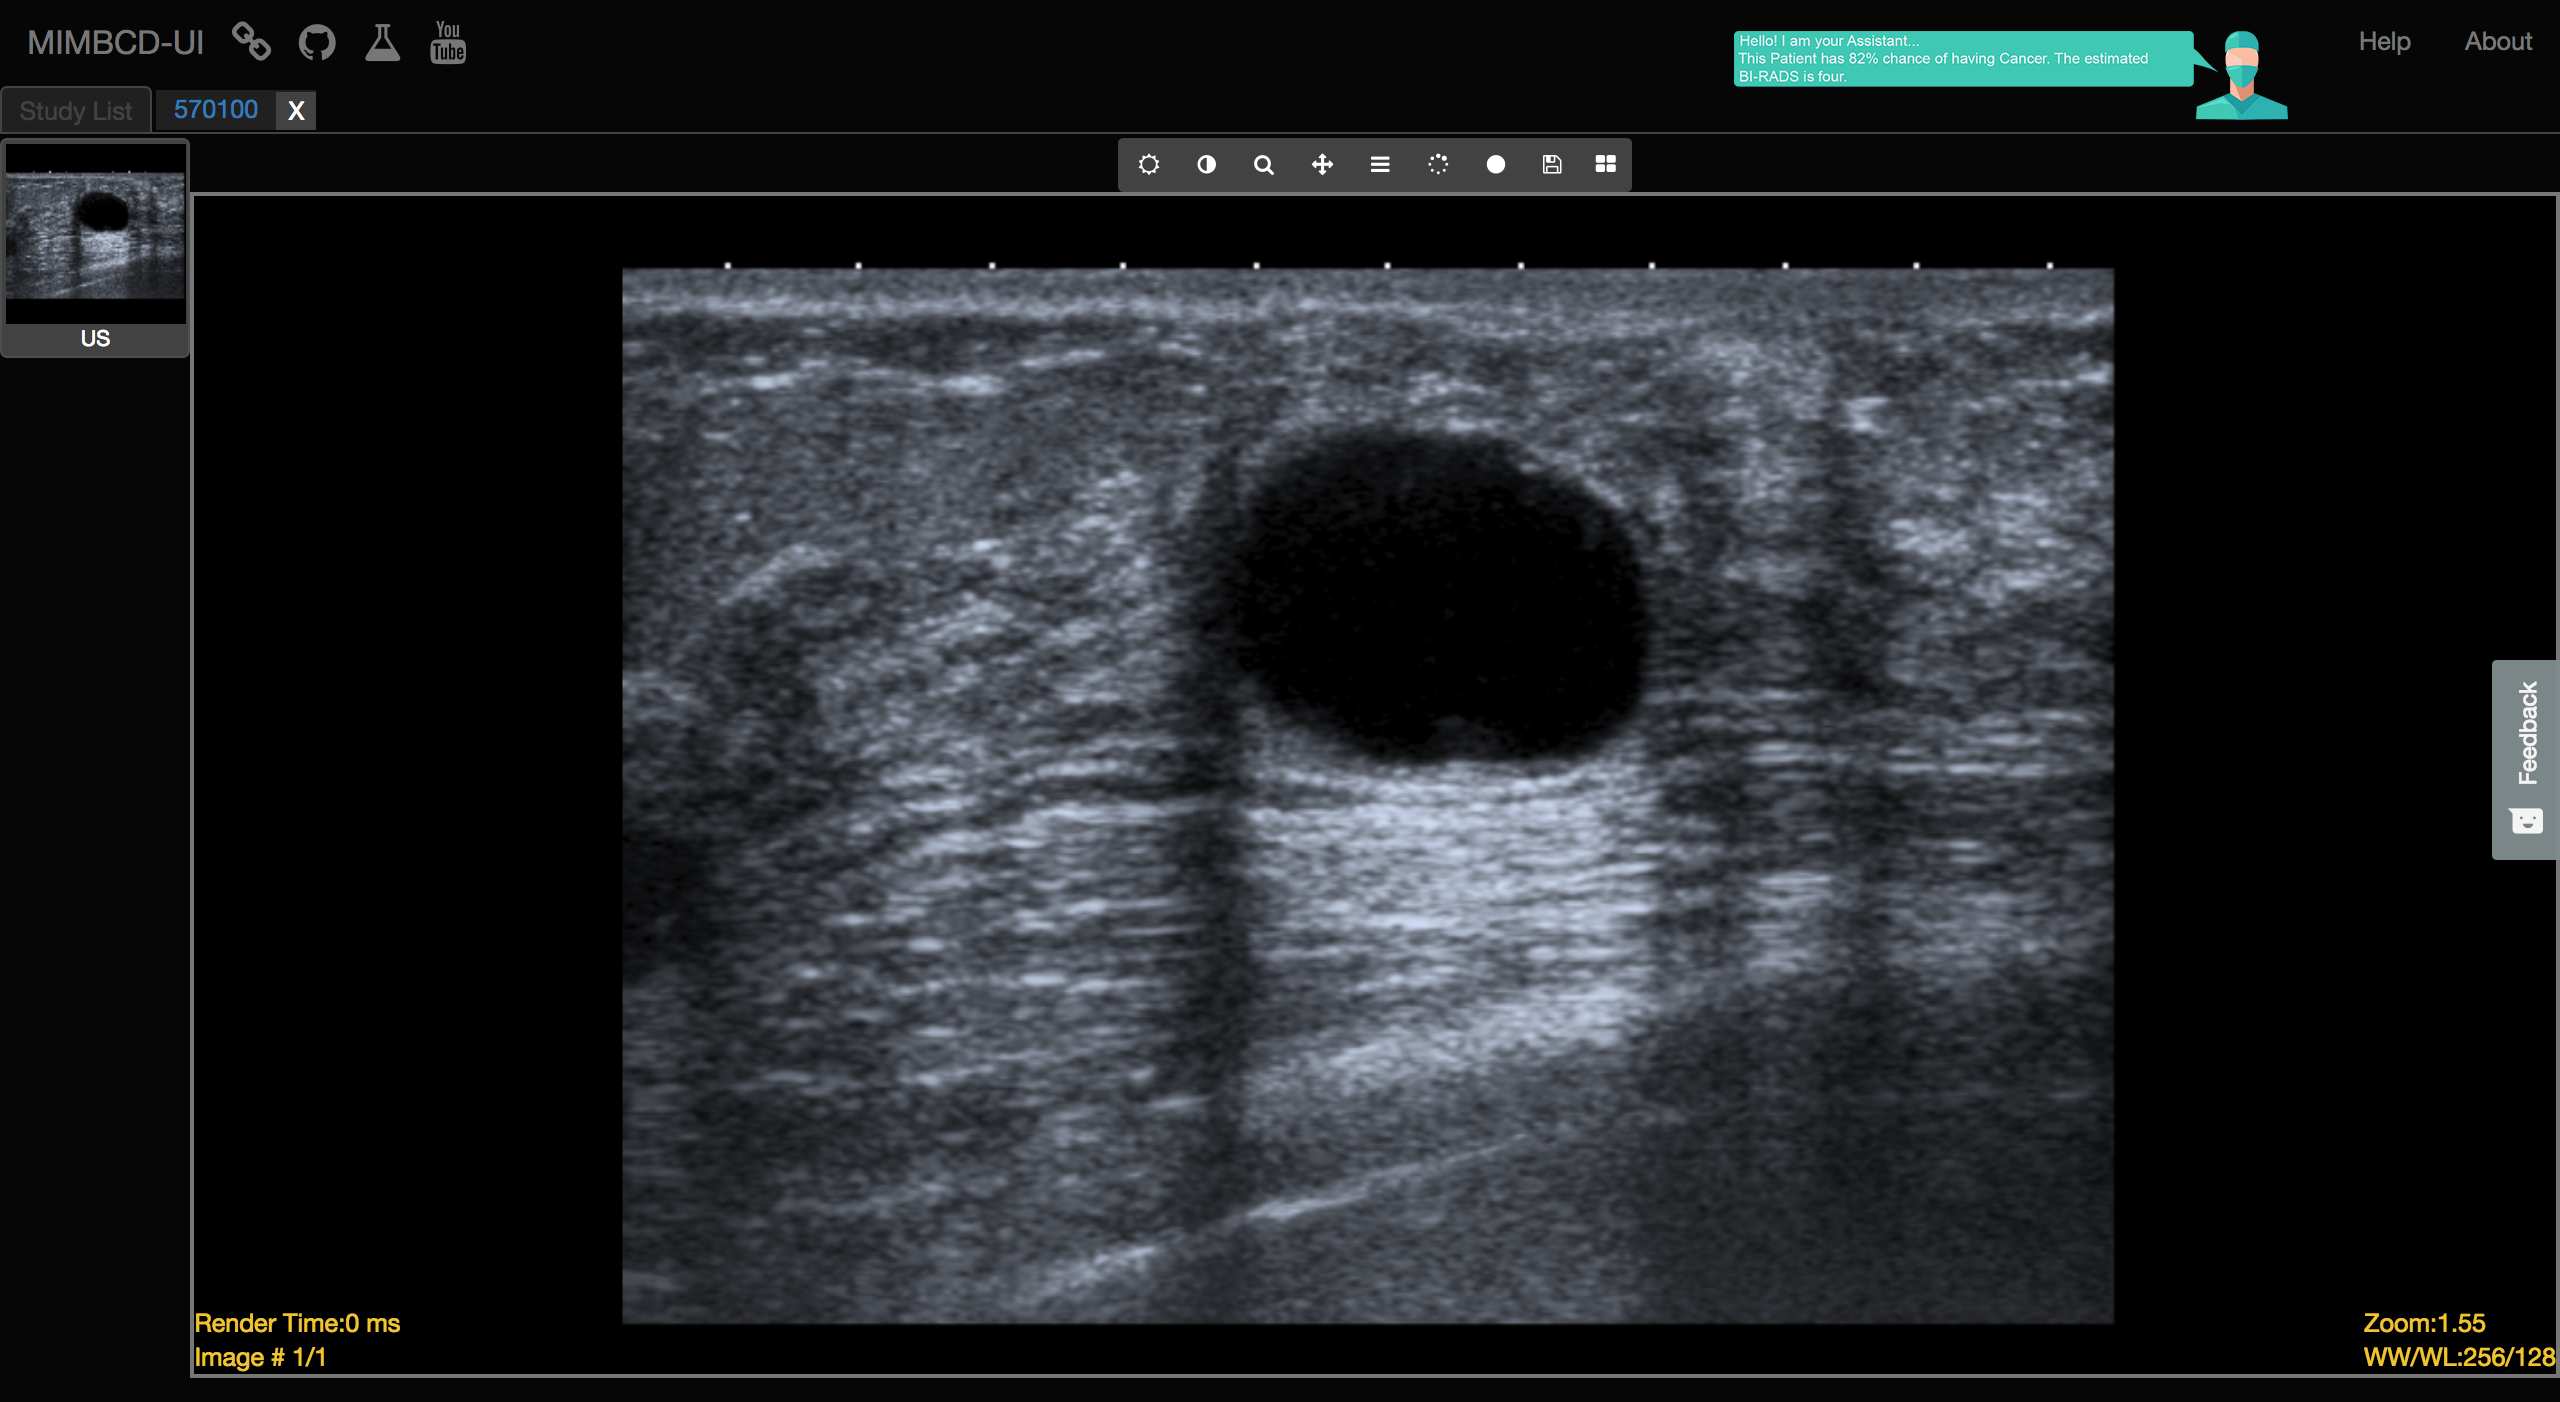
\includegraphics[width=\textwidth]{image_viewer}
\caption{Viewer of the \textbf{DICOM} images.}
\label{fig:image_viewer}
\end{figure}

\hfill

%%%%%%%%%%%%%%%%%%%%%%%%%%%%%%%%%%%%%%%%%%%%%%%%%%%

\subsection{Software}

To track our user interactions across our system, we are using \hyperlink{https://www.hotjar.com/}{Hotjar}. This tool is an analytic package allowing us to follow our users remotely. It also provides two critical pieces of functionality, among others, that can aid in remote user testing. First of all, the frequency areas allow us to see where users are clicking, tapping and scrolling on our system. Second, it records a video playback of the entire user session. The tool shows evidence of being useful for our studies while we successfully used it in the past. To record the task activities and the interview, we used \hyperlink{https://support.apple.com/downloads/quicktime}{QuickTime}~\cite{rowell2006internet}. The \hyperlink{https://support.apple.com/downloads/quicktime}{QuickTime} (\hyperlink{https://www.apple.com/}{Apple Computer}) tool is available on \hyperlink{https://www.apple.com/shop/buy-mac/macbook-pro}{MacBook Pro} for movie, audio and screen recording. Despite of have an overall of features, we just used it for our user's screen recording. It provides this functionalities at minimum requirements and compatible to our apparatus. Finally, we will take advantage of the \hyperlink{https://www.tobiipro.com/product-listing/tobii-pro-sdk/}{Tobii Pro SDK}~\cite{chatelain2018evaluation}, providing us the gaze information of the eye tracking device.

\clearpage